\section{UML Diagrams Overview}

\noindent
To provide a clearer understanding of the system's functionality and structure, two key UML diagrams were developed: a Use Case Diagram and a Sequence Diagram. These diagrams illustrate the system's behavioral aspects and the interactions between different actors and components.

\subsection{Use Case Diagram}

\noindent
The use case diagram (Figure~\ref{fig:use_case_diagram}) illustrates the major interactions between the different actors and the Void Training Platform system. It identifies six primary actors with distinct roles and responsibilities:

% \begin{itemize}
%     \item \textbf{Visitor}: Public users who can create accounts, view offers, and apply for opportunities
%     \item \textbf{Candidate}: Registered users who can track applications, apply to offers, and complete the selection process
%     \item \textbf{Trainee}: Accepted candidates who can work on final projects, manage personal VPS, access resources, and follow training programs
%     \item \textbf{Supervisor}: Staff members who manage educational resources, evaluate deliverables, manage training projects, and schedule interviews
%     \item \textbf{Administrator}: System administrators who manage users, assign roles, monitor resources, and handle system notifications
%     \item \textbf{Recruiter}: HR personnel responsible for managing internship offers, applications, and interviews
% \end{itemize}


\begin{figure}[H]
    \centering
    \makebox[\textwidth]{%
        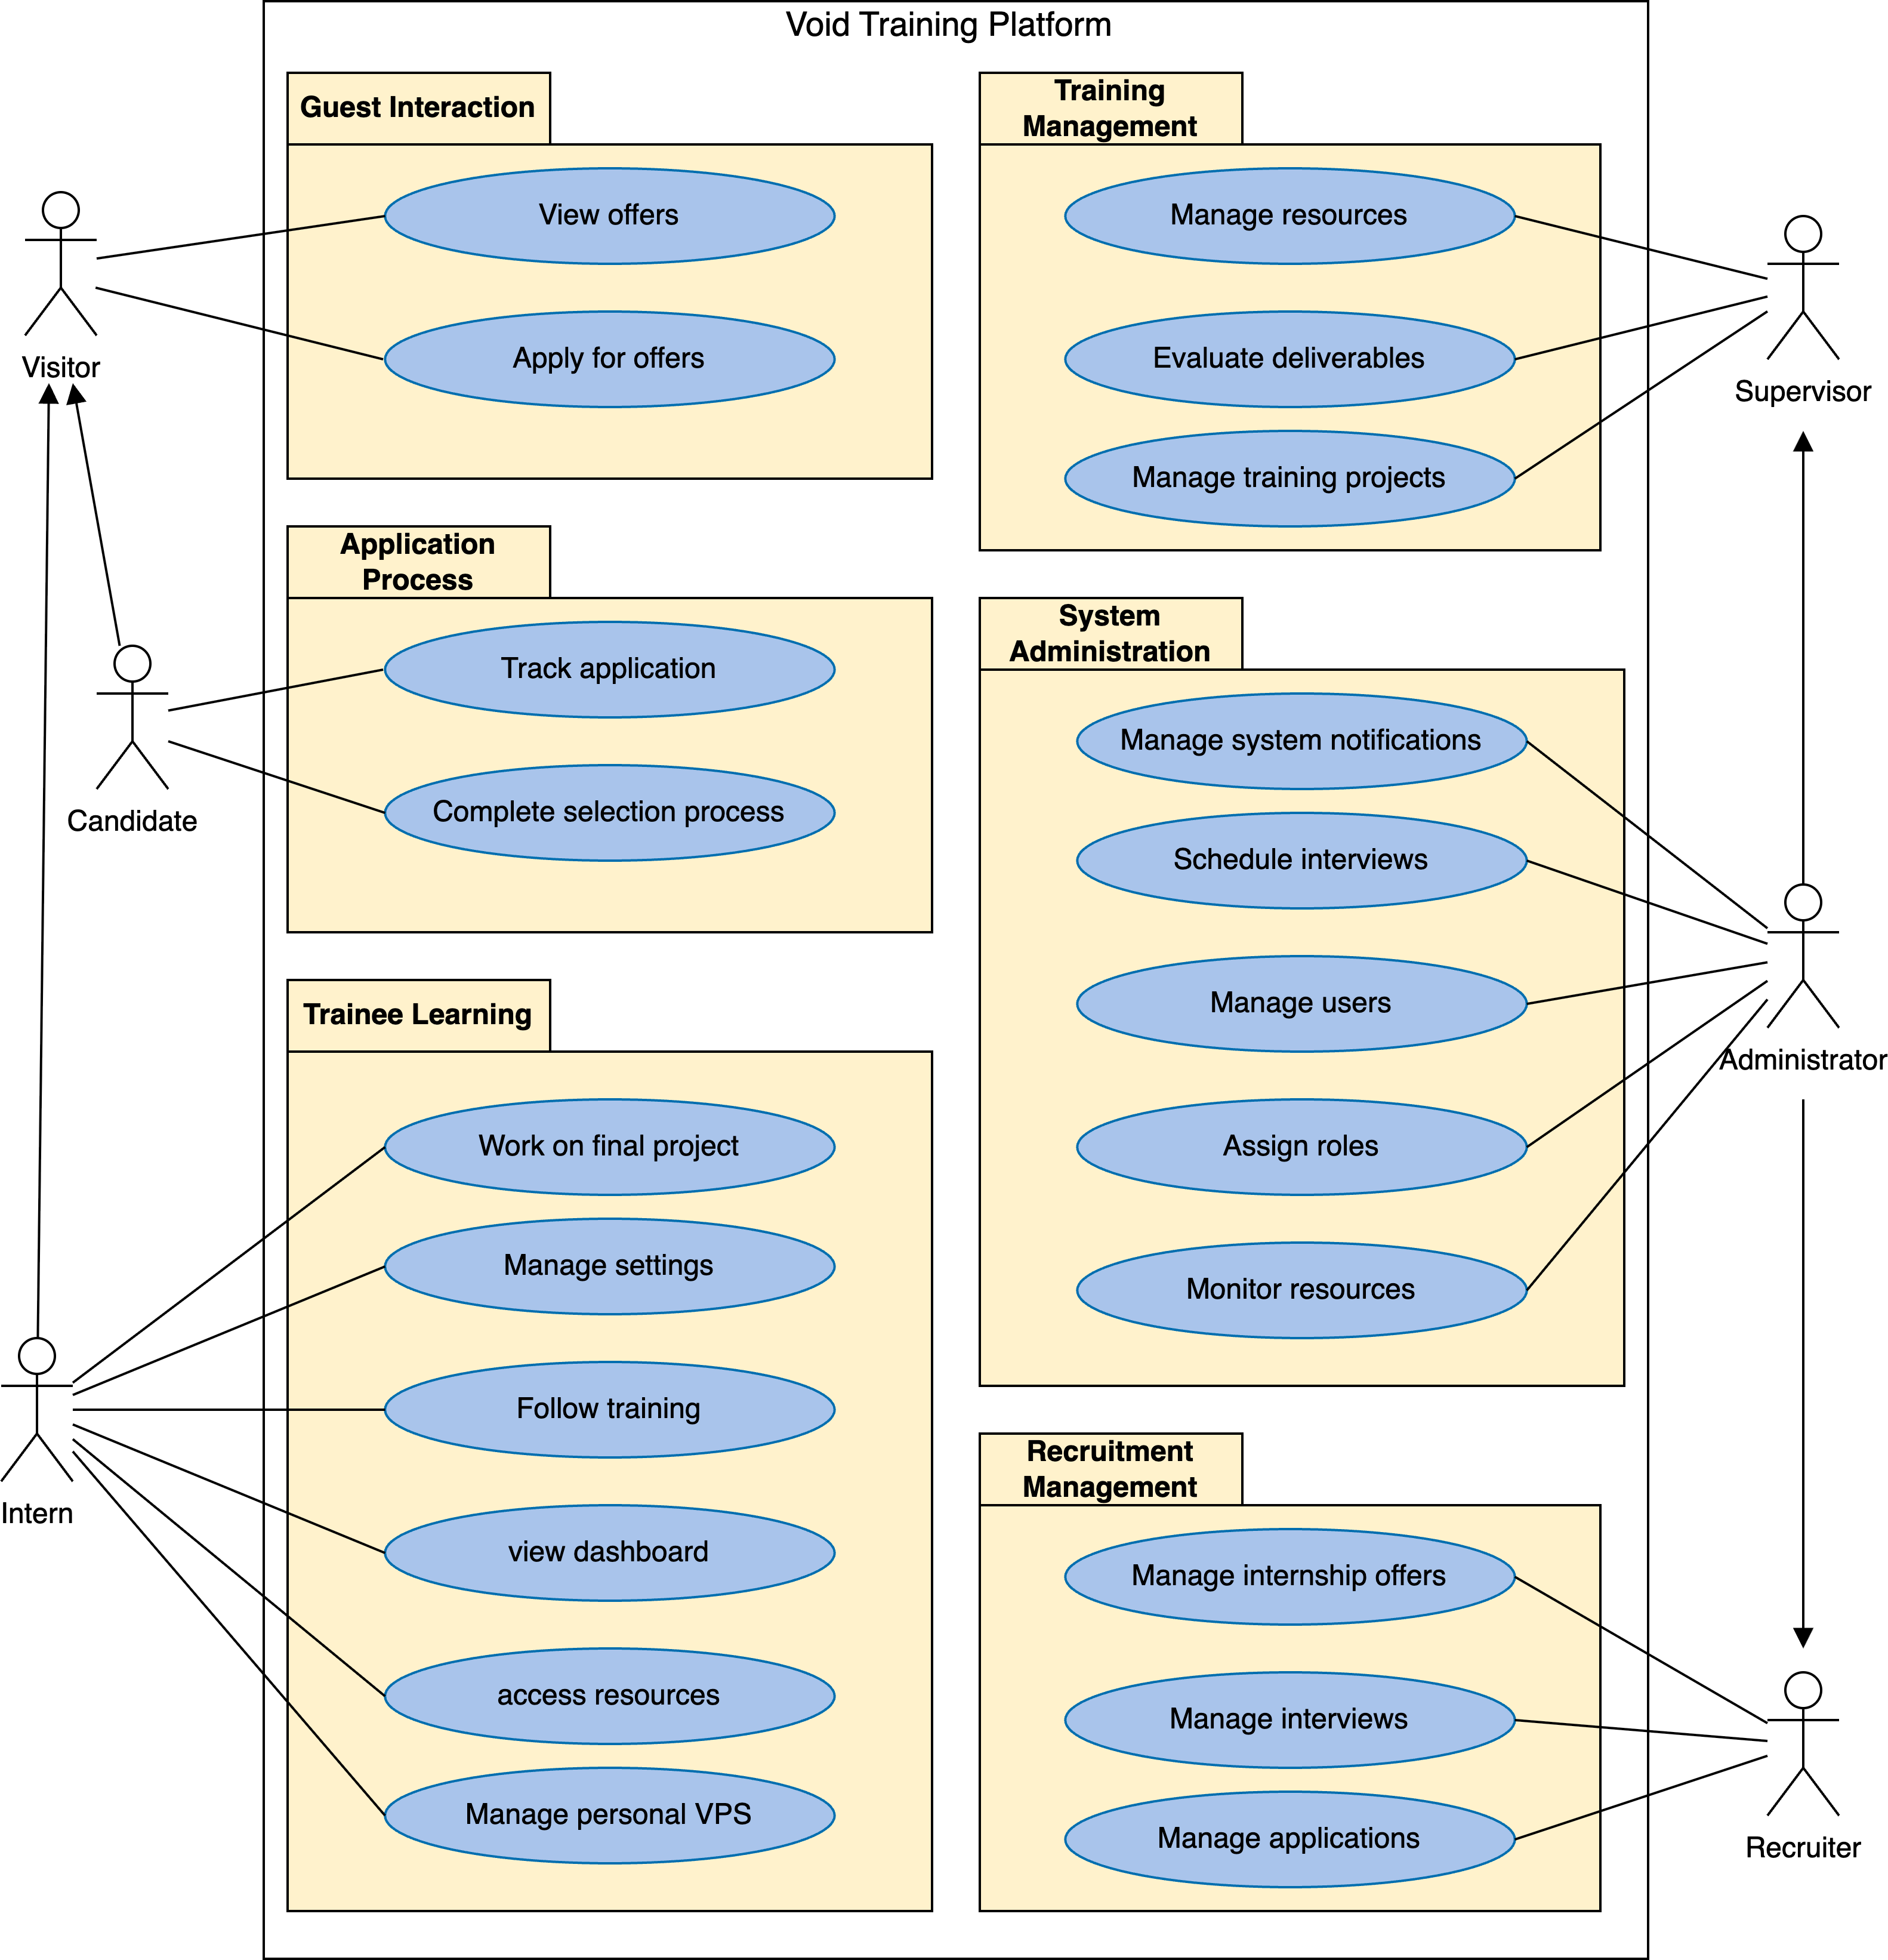
\includegraphics[width=1.1\textwidth]{images/usecase000.png}%
    }
    \caption{Use Case Diagram for the Intern Management Platform}
    \label{fig:use_case_diagram}
\end{figure}

\noindent
The Use Case Diagram provides a comprehensive overview of the system's functional requirements and user interactions within the Intern Management Platform. This diagram identifies six primary actors with distinct roles: Visitors who can browse and apply for opportunities, Candidates who track applications and complete selection processes, Trainees who access training resources and submit projects, Supervisors who manage educational content and evaluate deliverables, Administrators who handle system configuration and user management, and Recruiters who manage internship offers and interviews. The diagram illustrates key use cases including account management, training program participation, resource access, project submission and evaluation, and administrative oversight. This comprehensive view demonstrates how the platform supports the complete intern lifecycle from initial application through training completion.

\subsection{Sequence Diagram}

\noindent
The sequence diagrams represents the detailed interaction flow of the intern management platform, showing the communication between different system components. This diagram illustrates the technical architecture and data flow.

% The sequence diagram demonstrates the following key interaction patterns:

% \begin{itemize}
%     \item \textbf{Frontend-Backend Communication}: Shows how the Next.js frontend communicates with the Drupal backend through API proxy endpoints
%     \item \textbf{Authentication Flow}: Illustrates the Simple OAuth token-based authentication process for secure user sessions
%     \item \textbf{Data Processing Pipeline}: Demonstrates how candidate data flows through the system, from form submission to database storage
%     \item \textbf{Automated Workflows}: Shows automated processes including CV validation, account creation, and email notifications
%     \item \textbf{Assessment Integration}: Illustrates the technical test and challenge submission workflows
%     \item \textbf{Status Management}: Demonstrates how candidate status updates trigger appropriate notifications and system responses
% \end{itemize}

% Note about API proxy
\begin{figure}[H]
    \centering
    \makebox[\textwidth]{%
        \begin{minipage}{\textwidth}
            \textbf{Note:} All API calls in the following sequence diagrams use an API proxy to facilitate communication between the frontend and backend services.
        \end{minipage}%
    }
\end{figure}

% Sprint Management Sequence Diagram
\begin{figure}[H]
    \centering
    \makebox[\textwidth]{%
        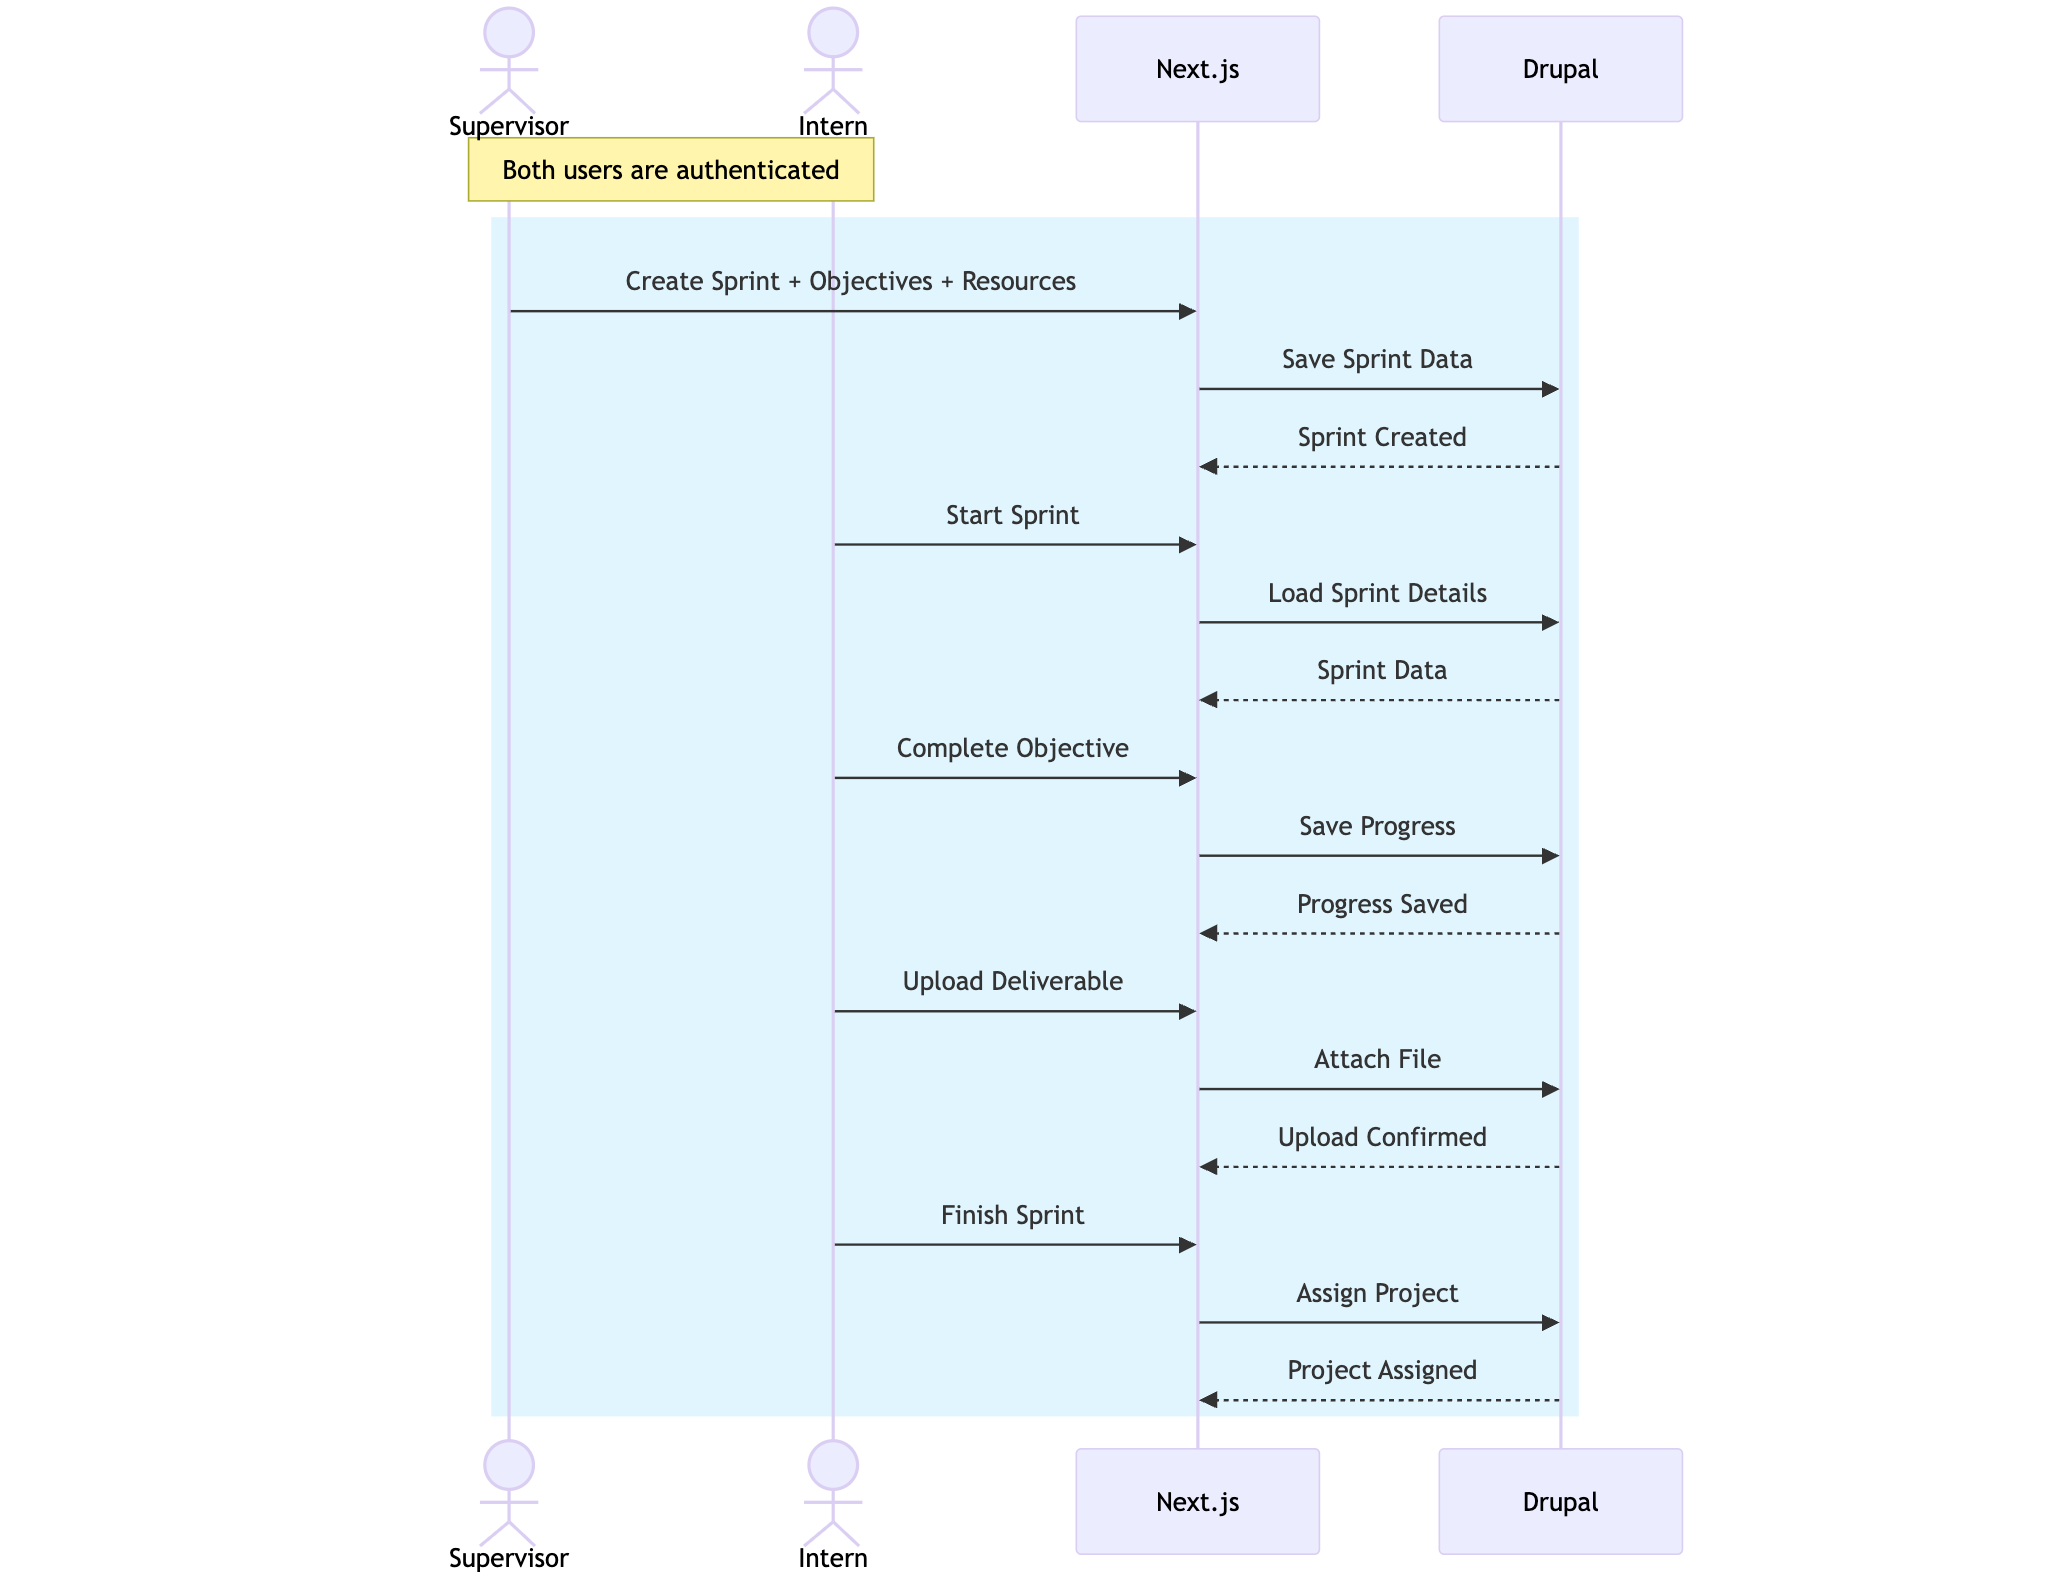
\includegraphics[width=1.3\textwidth]{images/mermaid-diagram-2025-06-15-010252.png}%
    }
    \caption{Sequence Diagram - Sprint Management Process Flow}
    \label{fig:sequence_diagram_sprint}
\end{figure}

\noindent
The Sprint Management Process Flow sequence diagram illustrates the complete lifecycle of sprint management within the training platform. This diagram demonstrates how supervisors create and manage training sprints, how trainees interact with sprint content, and how the system handles progress tracking and evaluation. The flow begins with sprint creation by supervisors, followed by trainee enrollment, content delivery, progress monitoring, and final evaluation. Key interactions include automated notifications, progress updates, and the integration between the frontend training interface and backend sprint management system.

% Project Management Sequence Diagram
\begin{figure}[H]
    \centering
    \makebox[\textwidth]{%
        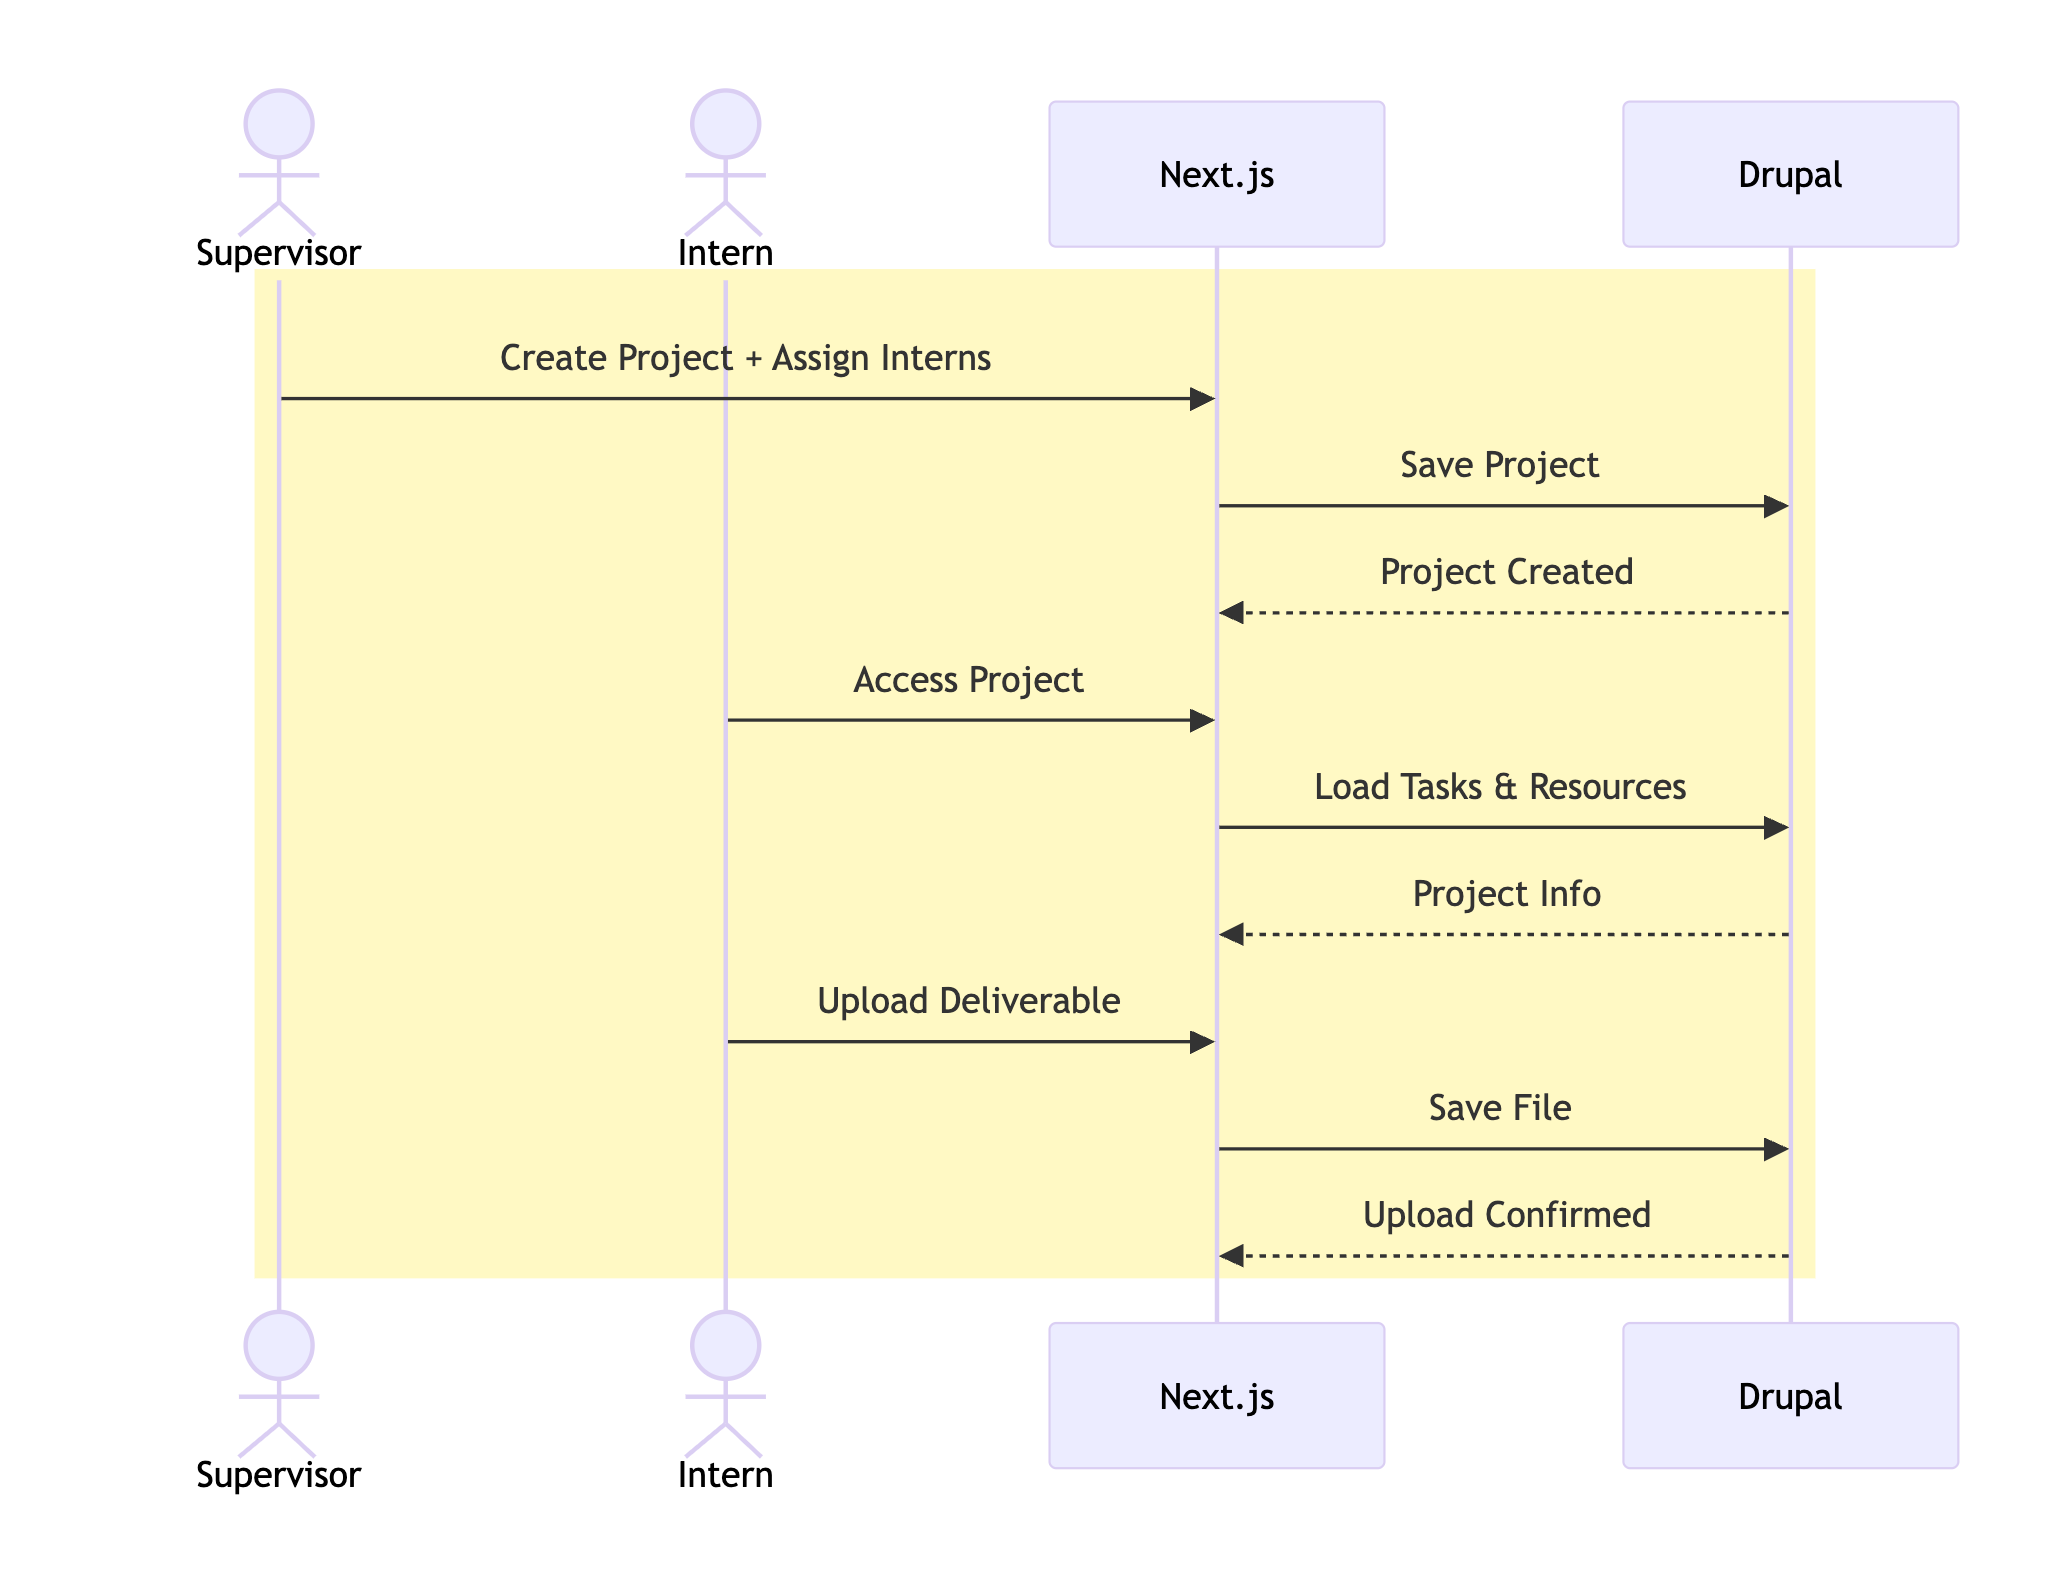
\includegraphics[width=0.9\textwidth]{images/mermaid-diagram-2025-06-15-175846.png}%
    }
    \caption{Sequence Diagram - Project Management Process Flow}
    \label{fig:sequence_diagram_project}
\end{figure}

\noindent
The Project Management Process Flow sequence diagram showcases the comprehensive project lifecycle management system. This diagram details how trainees submit project deliverables, how supervisors review and evaluate submissions, and how the system manages project status updates and feedback loops. The process includes project creation, milestone tracking, submission workflows, review processes, and final project evaluation. The diagram highlights the automated status updates, email notifications, and the seamless integration between the project submission interface and the backend evaluation system.

% Resource Management Sequence Diagram
\begin{figure}[H]
    \centering
    \makebox[\textwidth]{%
        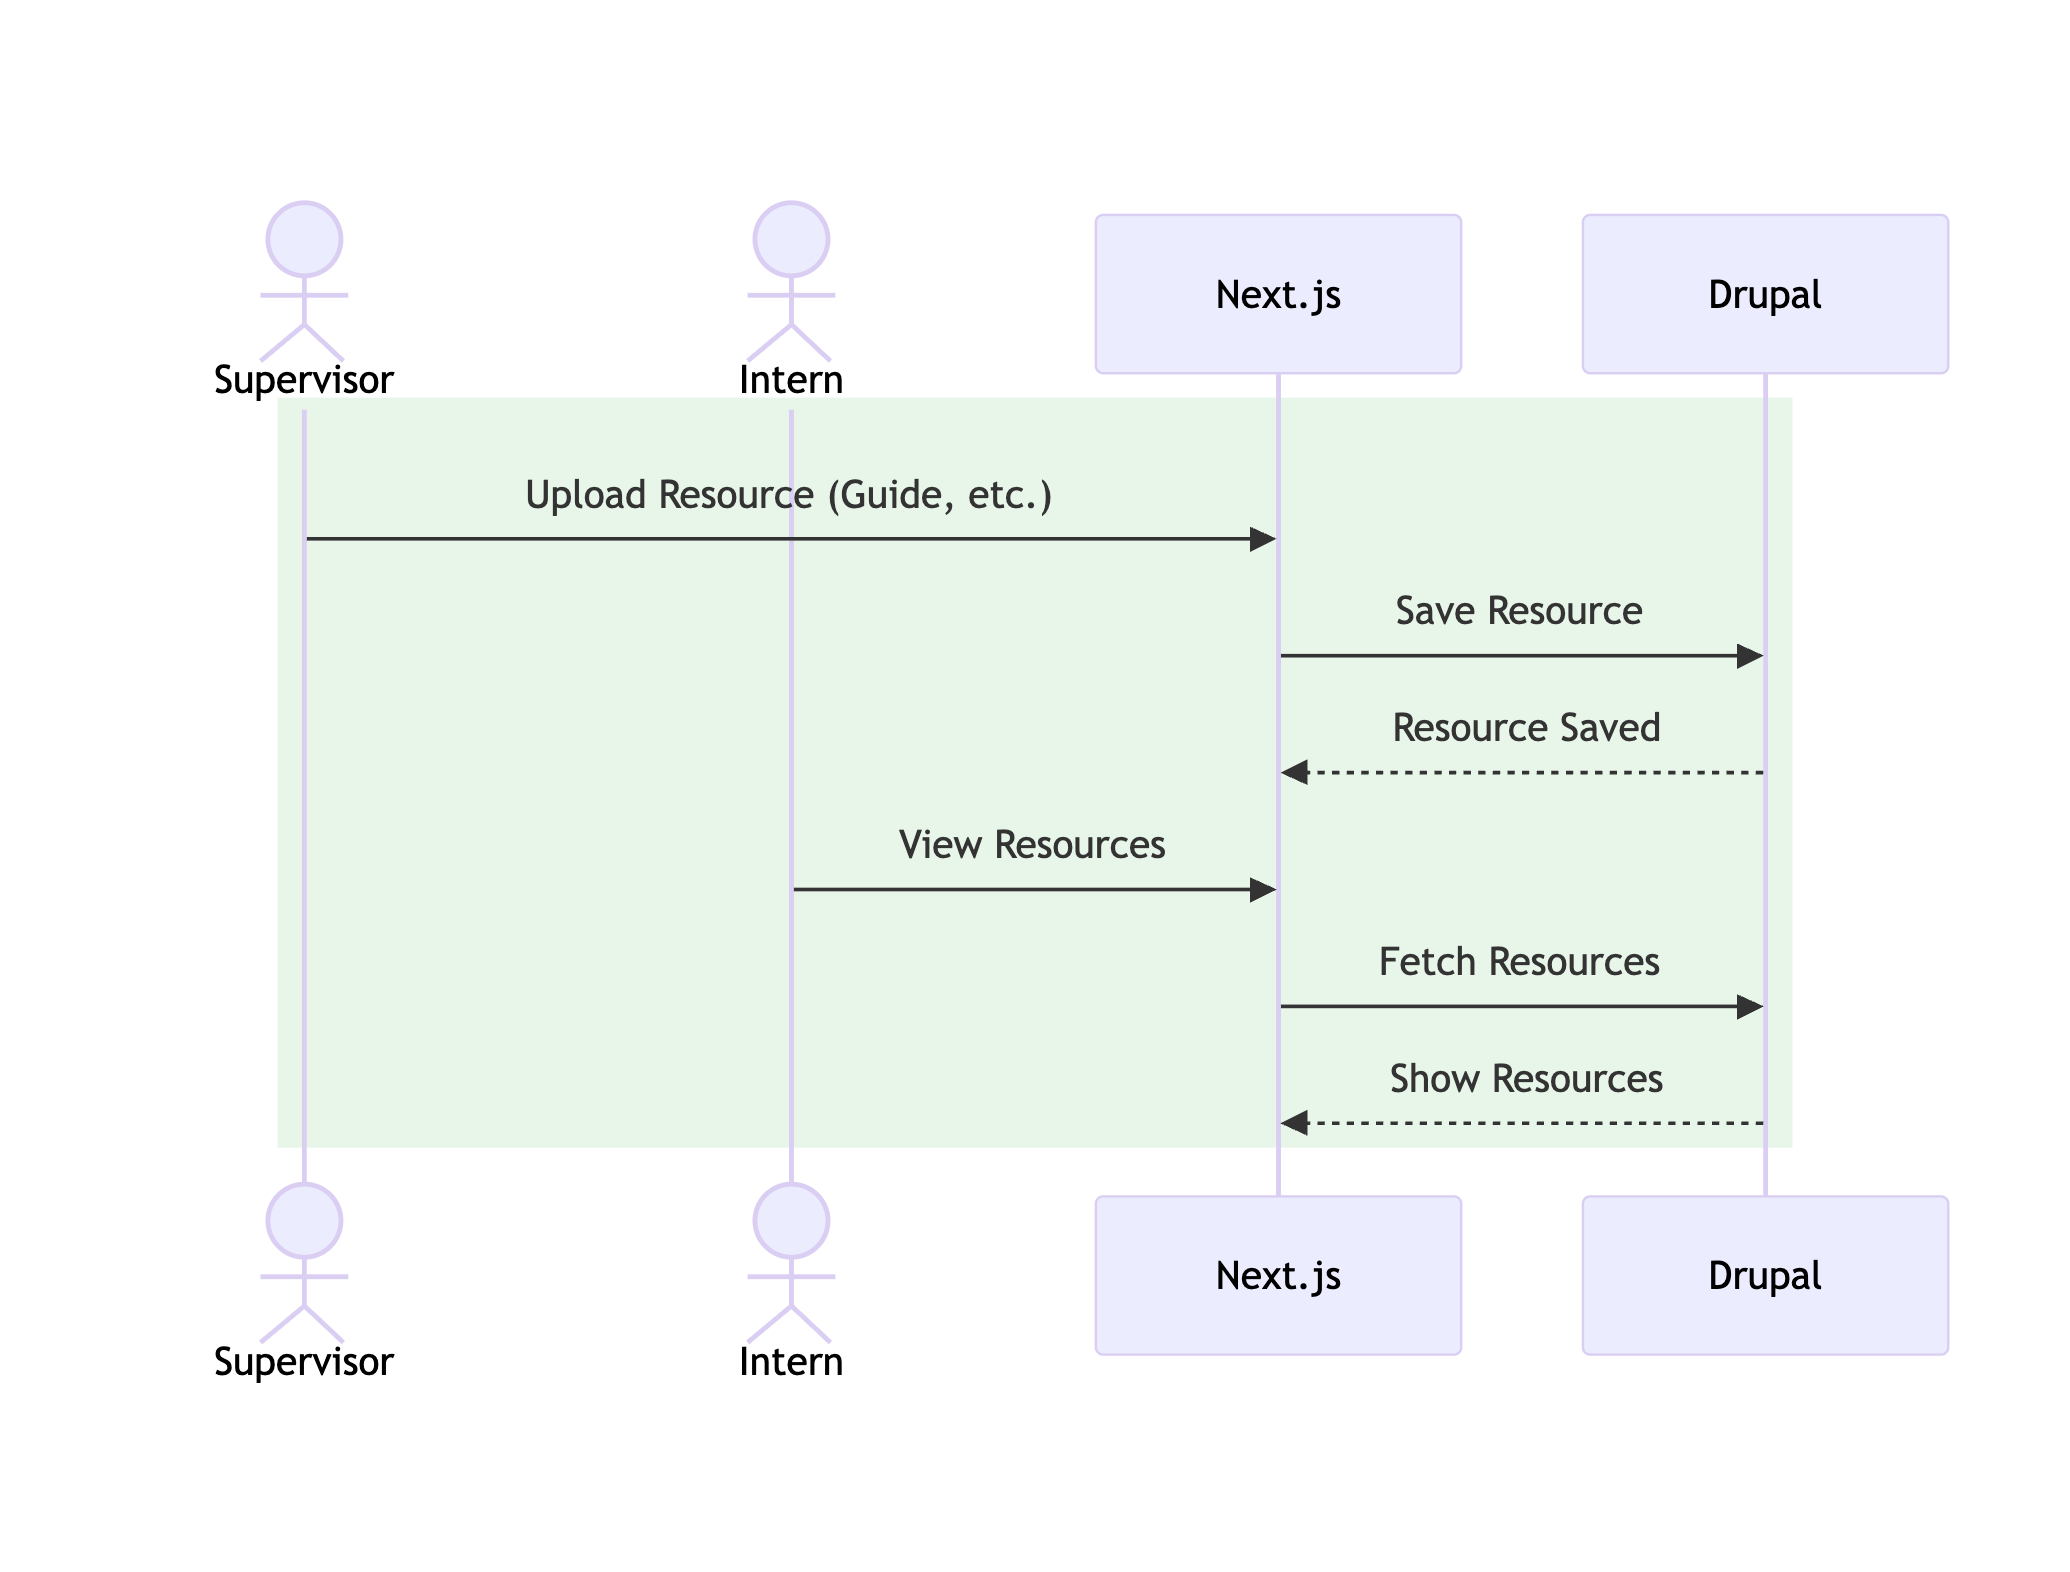
\includegraphics[width=0.9\textwidth]{images/mermaid-diagram-2025-06-15-141757.png}%
    }
    \caption{Sequence Diagram - Resource Management Process Flow}
    \label{fig:sequence_diagram_resource}
\end{figure}

\noindent
The Resource Management Process Flow sequence diagram demonstrates the complete resource lifecycle management within the training platform. This diagram illustrates how supervisors upload and organize educational resources, how trainees access and utilize these materials, and how the system manages resource categorization and access control. The flow encompasses resource creation, categorization, access management, usage tracking, and resource updates. The diagram emphasizes the role-based access control system, automated resource organization, and the integration between the resource library interface and the backend content management system.

\subsection{Class Diagram}

\noindent
The class diagram (Figure~\ref{fig:class_diagram}) presents the complete data model and entity relationships within the Intern Management Platform. This diagram illustrates the core entities, their attributes, and the relationships between different components of the system, providing a comprehensive view of the platform's structural design.

\begin{figure}[H]
    \centering
    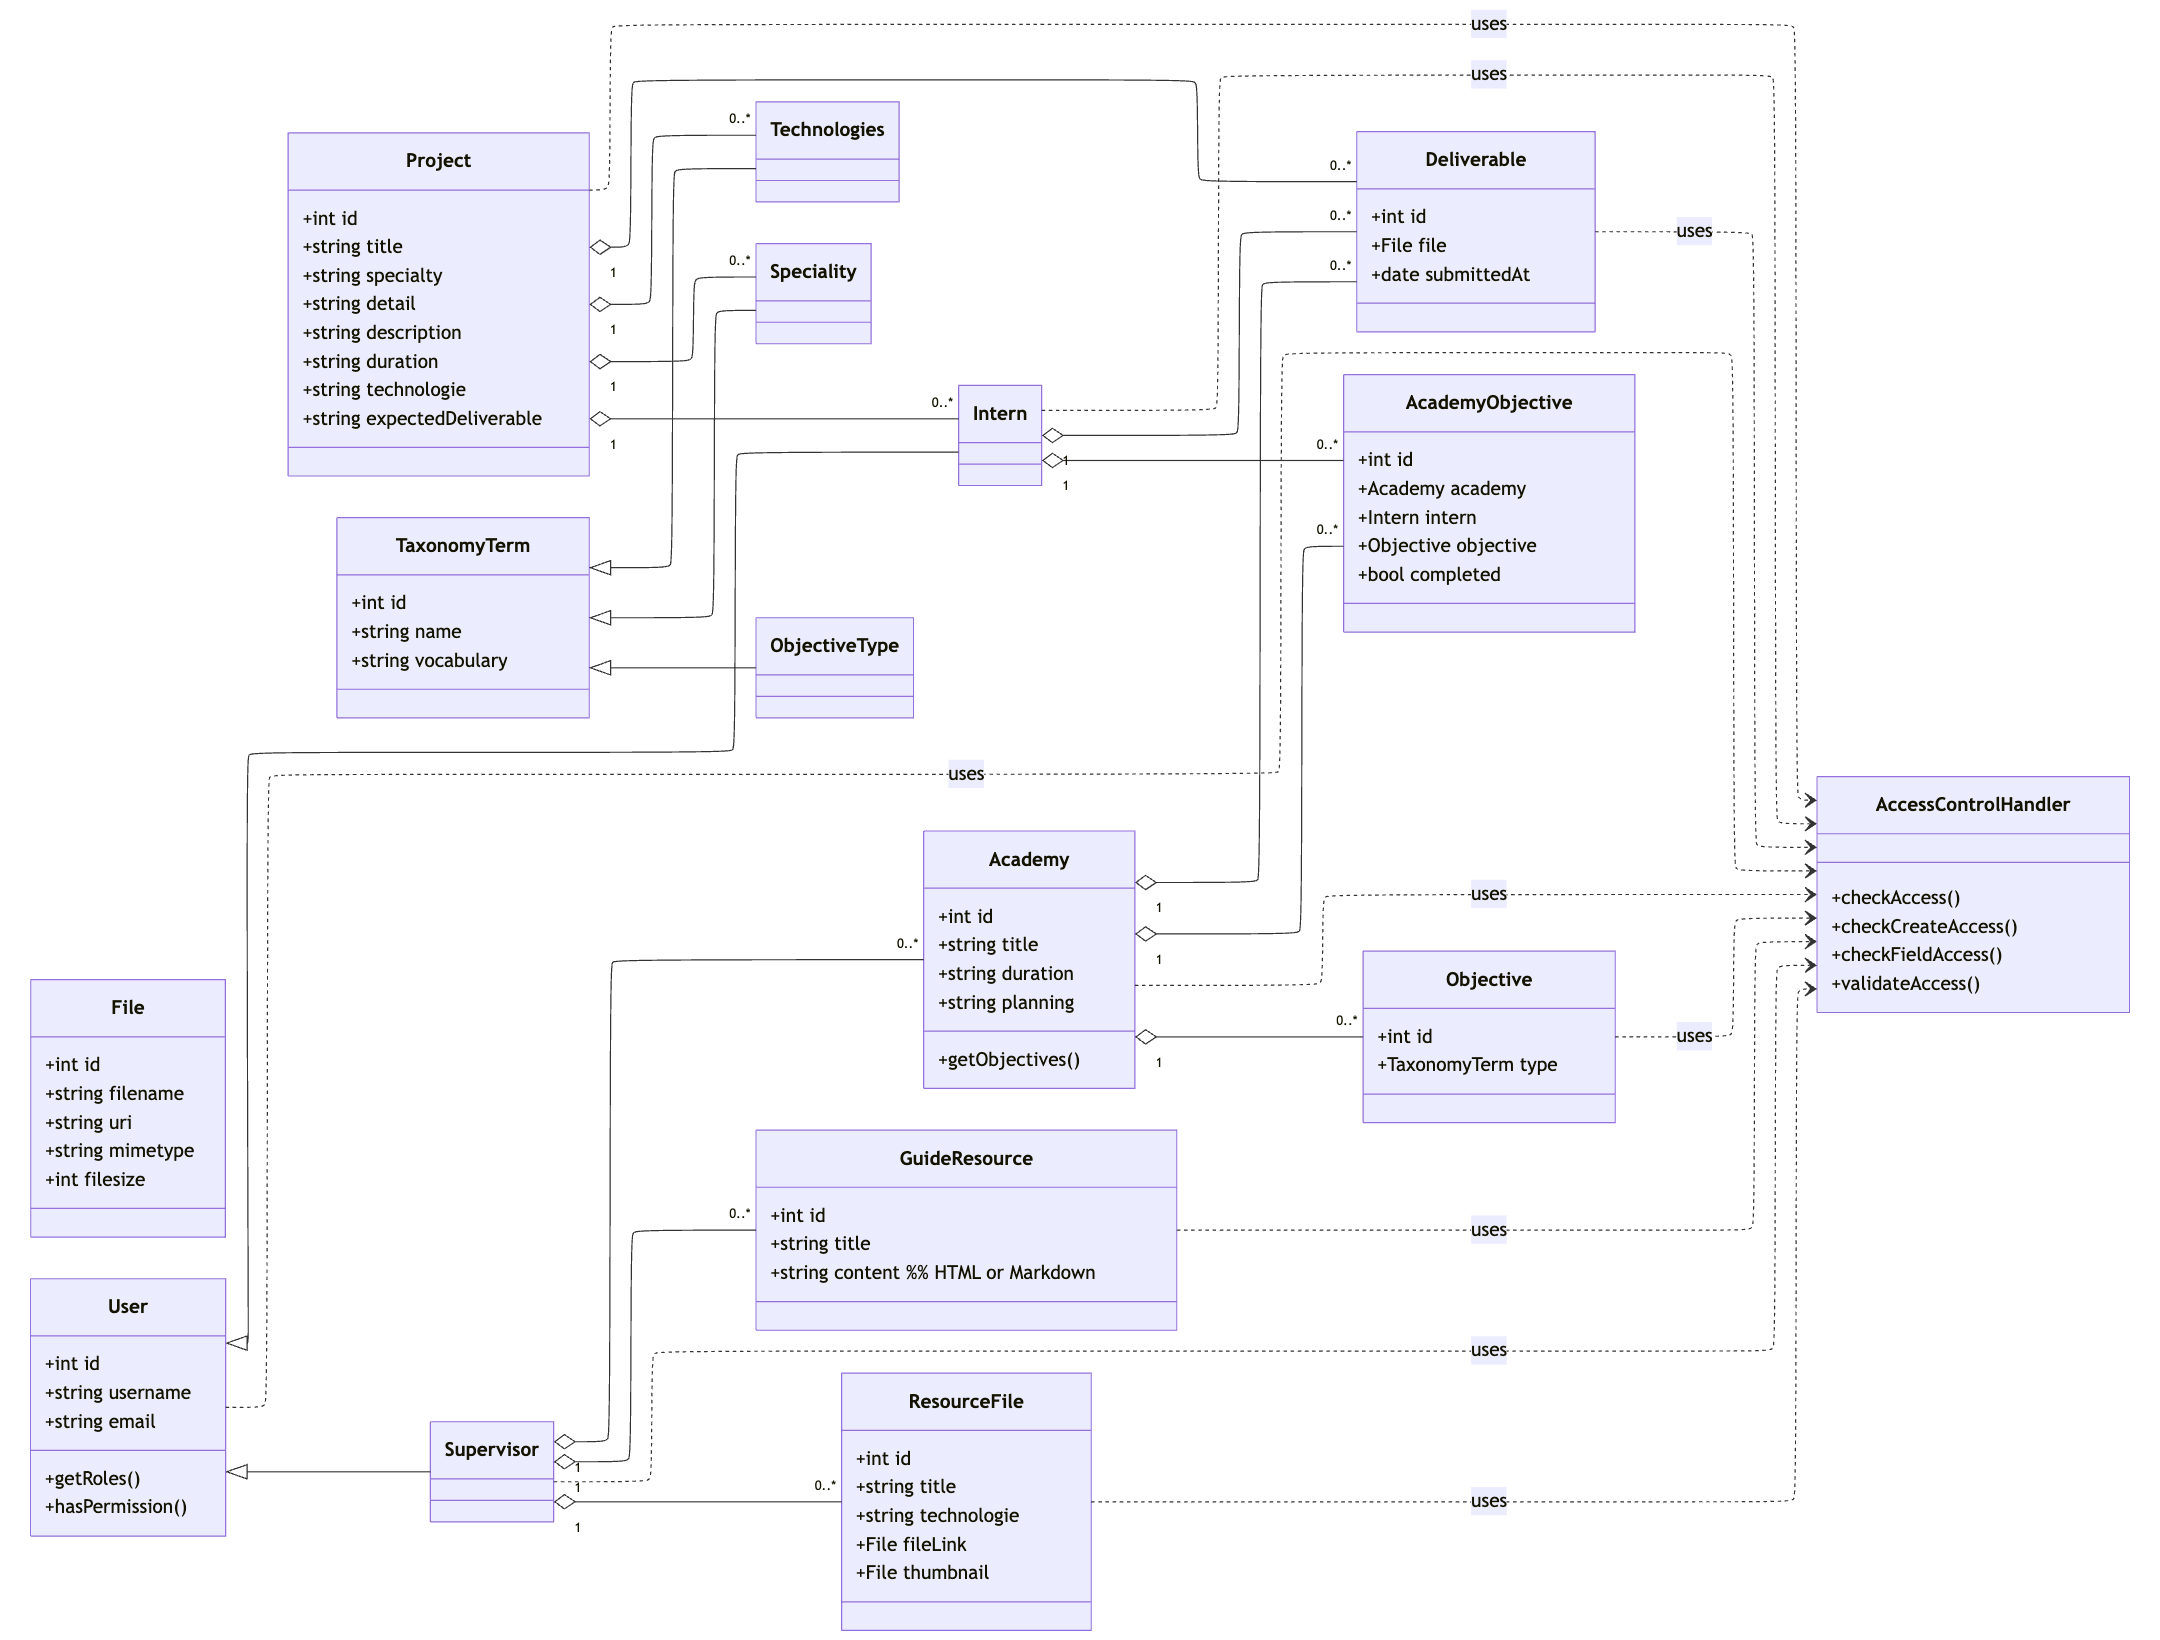
\includegraphics[angle=90,width=\textwidth,height=\textheight,keepaspectratio]{images/classfinalss.png}
    \caption{Class Diagram - System Entity Relationships and Data Model}
    \label{fig:class_diagram}
\end{figure}

\noindent
The Class Diagram provides a comprehensive view of the system's data architecture and entity relationships within the Intern Management Platform. This diagram illustrates the core entities including User management (with different roles like Trainee, Supervisor, Administrator), Training entities, and supporting entities. The diagram shows the relationships between entities, such as how Trainees are associated with multiple Sprints and Projects, how Supervisors manage Resources and evaluate Projects, and how the system handles Status tracking and automated Notifications. Key design patterns include role-based access control, hierarchical resource organization, and flexible status management systems that support the platform's training workflow requirements.

\subsection{Project Timeline Diagrams}

\noindent
Before diving into the main project implementation, it's important to note that a significant portion of time was dedicated to training and preparation. The team underwent an intensive two and a half months training phase to master the required technologies and methodologies, including Headless Drupal CMS, Next.js development, Agile workflows, DevOps practices, and CI/CD pipelines. This training phase was crucial for ensuring all team members were aligned on technical standards and development best practices.
\noindent
Following the training phase, the main project implementation was structured into six focused sprints, each targeting specific deliverables and building incrementally on previous work:

\begin{itemize}
    \item \textbf{Sprint 1: Setup} — Initial setup of the Vactory distribution and Drupal environment, along with the DevOps stack (OrbStack, Docker, EasyPanel).
    \item \textbf{Sprint 2: Main Website} — Development of the main website, including widget creation (Hero, FAQ, CTA, Process), job ads content types, taxonomies, and job offers listing modules.
    \item \textbf{Sprint 3: Training Platform (Backend)} — Implementation of backend features including training entities, project modules, resources management, access control, status taxonomy, and automated progress tracking.
    \item \textbf{Sprint 4: Training Platform (Frontend)} — Development of the training platform frontend, featuring the training space interface, resource library, status and objective trackers, project submission system, and progress monitoring dashboard.
    \item \textbf{Sprint 5: Admin Tools and Integration} — Development of admin dashboards, iframe review tools, role and permission setup, and the email notification system. Integration of all modules and finalization of admin features.
    \item \textbf{Sprint 6: Testing, Documentation, and Deployment} — Comprehensive testing and debugging (frontend and backend), CI/CD pipeline setup, Docker Compose finalization, and preparation of final documentation and delivery.
\end{itemize}

\begin{figure}[H]
    \centering
    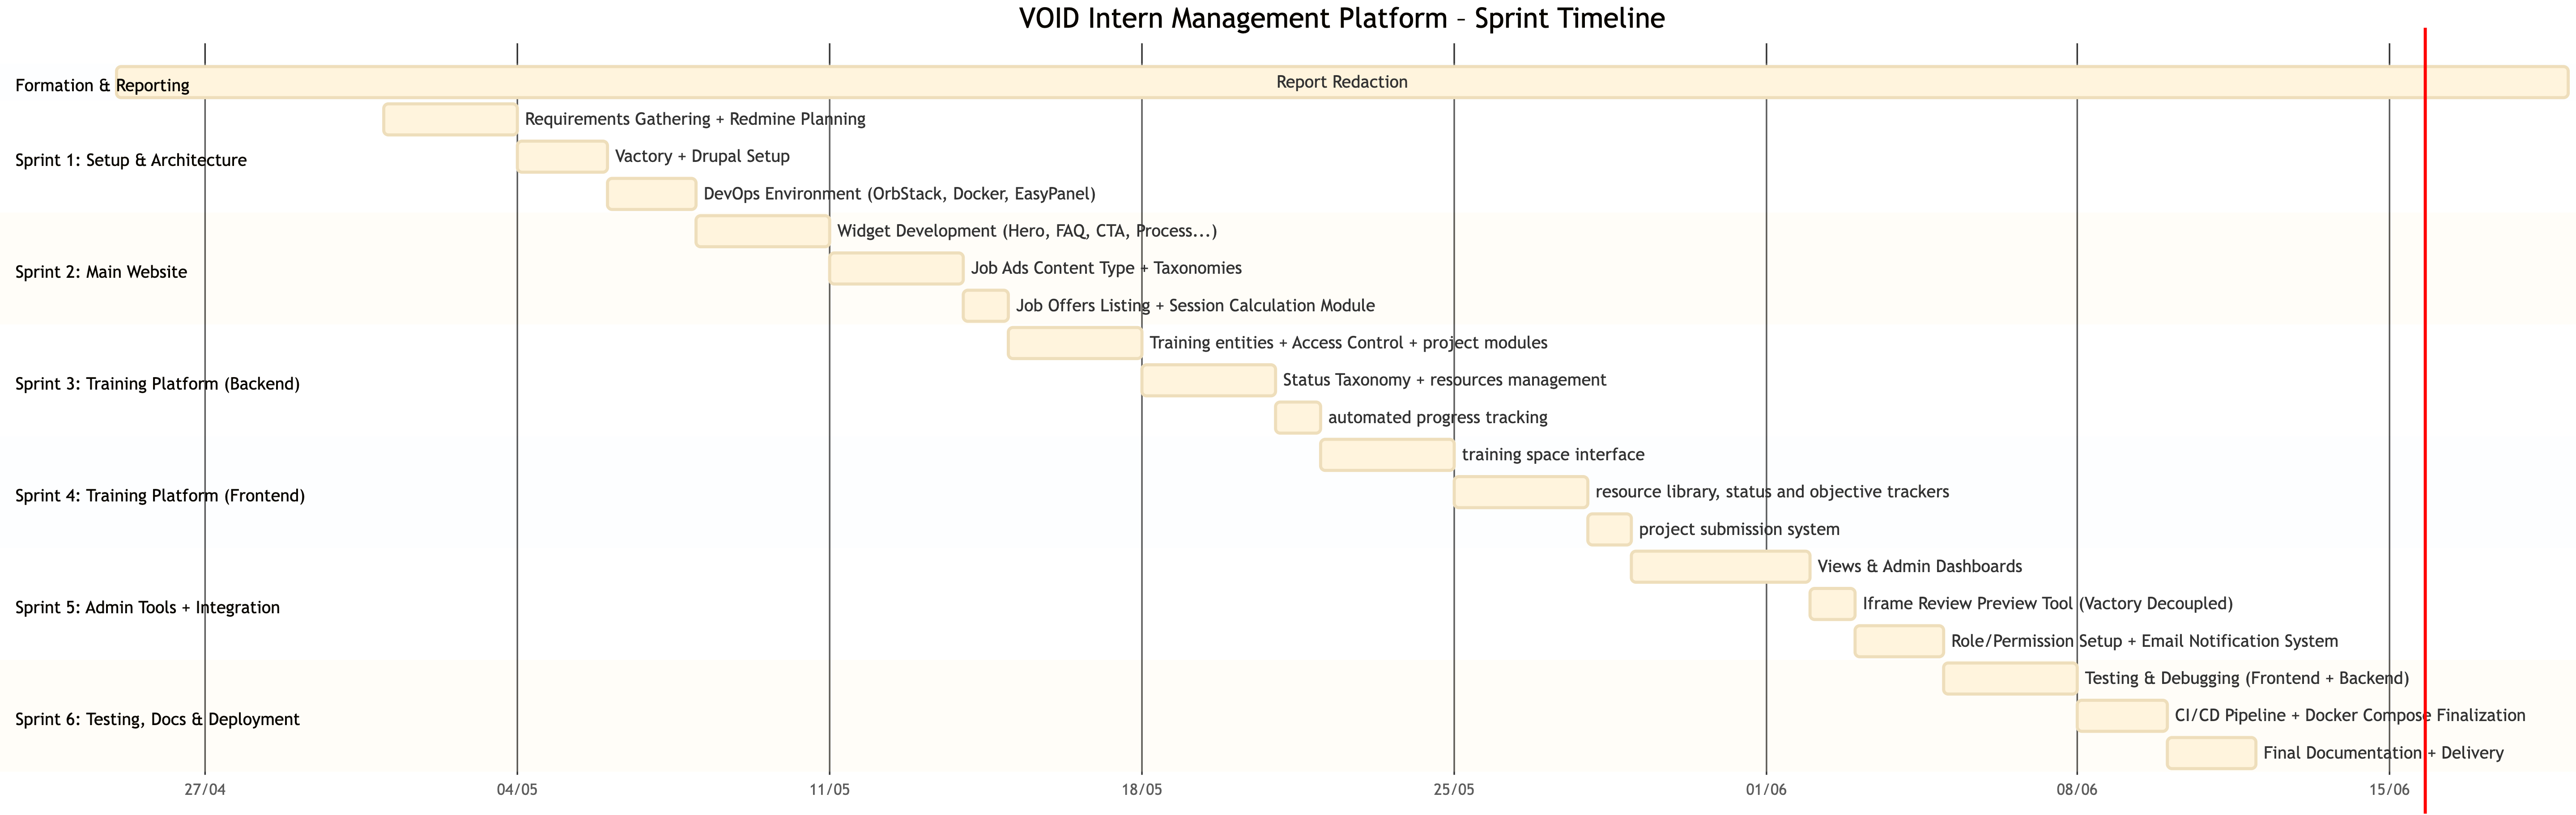
\includegraphics[angle=90,width=\textwidth,height=\textheight,keepaspectratio]{images/gant-wwi.png}
    \caption{Project Implementation Gantt Chart - VOID Intern Management Platform Sprint Timeline (6 Weeks)}
    \label{fig:gantt_project}
\end{figure}
